
\documentclass[../main]{subfiles}
\ifSubfilesClassLoaded{
    \dominitoc
    \tableofcontentsfile
    \setcounter{page}{1} 
    \setcounter{chapter}{1}
}{}
\begin{document}
\chapter{Modèle d'architecture CxSOM}{\label{chap:modele}}
\graphicspath{{03-SOM/},{./}}
\minitoc

\section{Introduction}

Nous proposons dans cette thèse un modèle d'architecture non-hiérarchique de cartes auto-organisatrices, CxSOM. 
\`A partir de ces architectures, nous cherchons à apprendre des relations entre des données issues de plusieurs modalités. 
On souhaite que ce modèle soit générique, permettant de construire n'importe quel forme et taille d'architecture, et ayant la possibilité d'intégrer des connexions récurrentes. 
Notre démarche est d'abord de proposer un modèle de calcul général à base de cartes auto-organisatrices~; des applications plus spécifiques pourront être développées à partir de cette méthode.

Nous avons défini une \emph{architecture} de carte par un réseau composé de plusieurs modules qui sont chacun une carte de Kohonen et dans lequel des connexions sont définies entre ces modules. Ces connexions sont orientées: on parle d'une connexion d'une carte A vers une carte B. Le but de ces connexions est de coupler l'apprentissage de plusieurs cartes.
Sur une telle architecture, on peut construire un graphe $G$ orienté, dont les n\oe{}uds sont des cartes. La connexion d'une carte A vers une carte B est indiquée par la présence d'une arête de A vers B. 
On appelle architecture \emph{non-hiérarchique} une architecture pour laquelle le graphe $G$ n'est pas un arbre: il présente des boucles. Un exemple d'architecture non-hiérarchique est représenté en figure~\ref{fig:archi_non_hierarchique}. Certaines cartes sont connectées dans les deux directions, d'autres en boucle. Dans cette thèse, nous cherchons à utiliser de telles architectures non-hiérarchiques pour des tâches de mémoire associative.
Chaque carte de l'architecture cherche d'une part à apprendre une représentation de l'entrée $A,B,C,D,E$ ou $F$ qui lui est fournie. 
Lorsque ces entrées présentent des dépendances les unes aux autres, l'architecture dans sa globalité doit également, d'une façon ou d'une autre, extraire les relations, les dépendances, existant entre les distributions de données. Cet apprentissage des relations est au c\oe{}ur de cette thèse, sa partie expérimentale se concentrant sur les représentations et indicateurs mettant en valeur l'apprentissage de ces relations puis en les utilisant sur différents ensemble de données d'entrée.

Dans ce chapitre, nous détaillons d'abord le modèle CxSOM que nous avons développé et étudié durant cette thèse. Il permet de construire des architectures non-hiérarchiques de cartes auto-organisatrices. 
Nous présentons en premier lieu le formalisme et les notations d'une carte de Kohonen classique, dont sont dérivées les cartes auto-organisatrices utilisées dans les architectures CxSOM. 
Nous expliquons ensuite les choix de développement sur lesquels nous nous sommes appuyée pour développer le modèle. Nous présentons le modèle sur un exemple d'architecture à deux cartes, puis nous le formalisons pour le cas général de $n$ cartes connectées au sein d'une architecture.

\begin{figure}
\centering
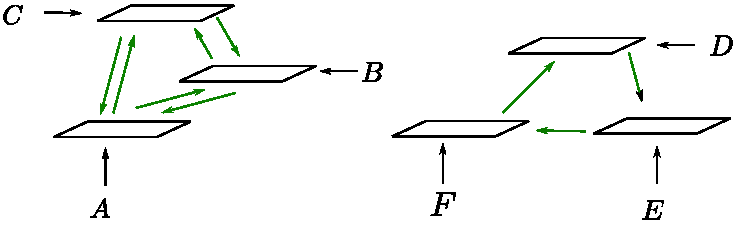
\includegraphics[width=0.6\textwidth]{architecture.pdf}
\caption{Deux exemples d'architectures \emph{non-hiérarchiques} à 3 cartes de Kohonen faisant figurer des connexions réciproques ou des boucles au sein de l'architecture.
Les entrées fournies au cartes sont $A,B,C,D,E,F$ quelconques.}
\label{fig:archi_non_hierarchique}
\end{figure}


\section{Carte de Kohonen classique}\label{sec:kohonen}

Chaque carte de Kohonen d'une architecture CxSOM est directement dérivée de l'algorithme d'une carte de Kohonen classique introduite en \cite{Kohonen1982}. Cet algorithme et ses dérivés sont décrits en détail par T. Kohonen dans son ouvrage~\cite{Kohonen1995SelfOrganizingM}. Le principe général d'une carte de Kohonen a été décrit dans le chapitre précédent; nous définissons ici plus précisément le modèle et les équations qui serviront de base pour la définition de l'algorithme CxSOM.

\subsection{Algorithme et notations}

Une carte de Kohonen est un graphe, généralement une ligne 1D ou une grille 2D de $N$ n\oe{}uds. Nous utiliserons dans cette thèse des cartes en une et deux dimensions, c'est-à-dire des lignes et des grilles. Les notations et le modèle présentés ici sont toutefois applicables à des cartes de dimensions et topologie quelconques.

L'algorithme et les notations sont résumés en figure~\ref{fig:one_map_not}. Une entrée fournie à une carte de Kohonen est notée $\inpx_t$, tirée dans un espace d'entrée $\mathcal{D}$. \`A chaque n\oe{}ud de la carte est associé un poids $\w_e \in D$, appelé aussi prototype. Sa \emph{position} dans la carte est indexée par $p$. Nous choisissons d'indexer les positions dans $[0,1]$~: l'ensemble des positions $p$ est donc un ensemble de points discrets entre $0$ et $1$. L'ensemble des poids est noté $\{\w_e(p), p \in \{0,\cdots,\frac{i}{N-1}, \cdots, 1\}\}$, avec $i$ l'indice entier d'un noeud de la carte. On peut faire la même discrétisation de l'espace $[0,1]^2$ pour une carte en 2D.

Une étape $t$ de l'algorithme de mise à jour d'une carte de Kohonen contient les étapes suivantes:
\begin{enumerate}
\item\label{enum:inp} Une entrée $\inpx_t$ est tirée et présentée à la carte.
\item\label{enum:act} Une \emph{activité} $a_e(\inpx_t,p)$ est calculée dans la carte pour chaque noeud de position $p$. La fonction d'activité que nous utiliserons dans cette thèse est une activation gaussienne:
\begin{equation}\label{eq:act1som}
a_e(\inpx_t,p) = \exp{\frac{-\lVert \inpx_t-\w\ext(p) \rVert ^2}{2\sigma^2}}
\end{equation}
\item\label{enum:bmu} L'unité ayant l'activité maximale est la \emph{Best Matching Unit} de la carte. Sa position est notée $\bmu_t$.
\item Chaque poids $\w_e$ est déplacé vers l'entrée $\inpx$. Le déplacement est pondéré par une \emph{fonction de voisinage} $H(\bmu,p)$. Cette fonction est maximale en $p = \bmu$ et décroissante autour de cette position. Dans notre étude, la fonction de voisinage est triangulaire, maximale en $\bmu_t$, linéairement décroissante sur un \emph{rayon de voisinage} noté $h_e$ et nulle sinon.
\begin{equation}
\w_e(p,t+1) = \w_e(p,t) + \alpha H(\bmu_t,p)(\inpx_t - \w_e(p,t))
\label{eq:update}
\end{equation}
\end{enumerate}

L'étape de calcul d'activité est déjà une modification de l'algorithme original de Kohonen.
Dans la version classique, on calcule plutôt les distances entre l'entrée et les poids $\lVert \inpx_t - \w_e(p) \rVert$, et le BMU est choisi comme l'unité dont le poids présente la plus petite distance à l'entrée. 
Ici, on prendra comme BMU l'unité ayant l'activité la plus élevée.

\begin{figure}
\centering
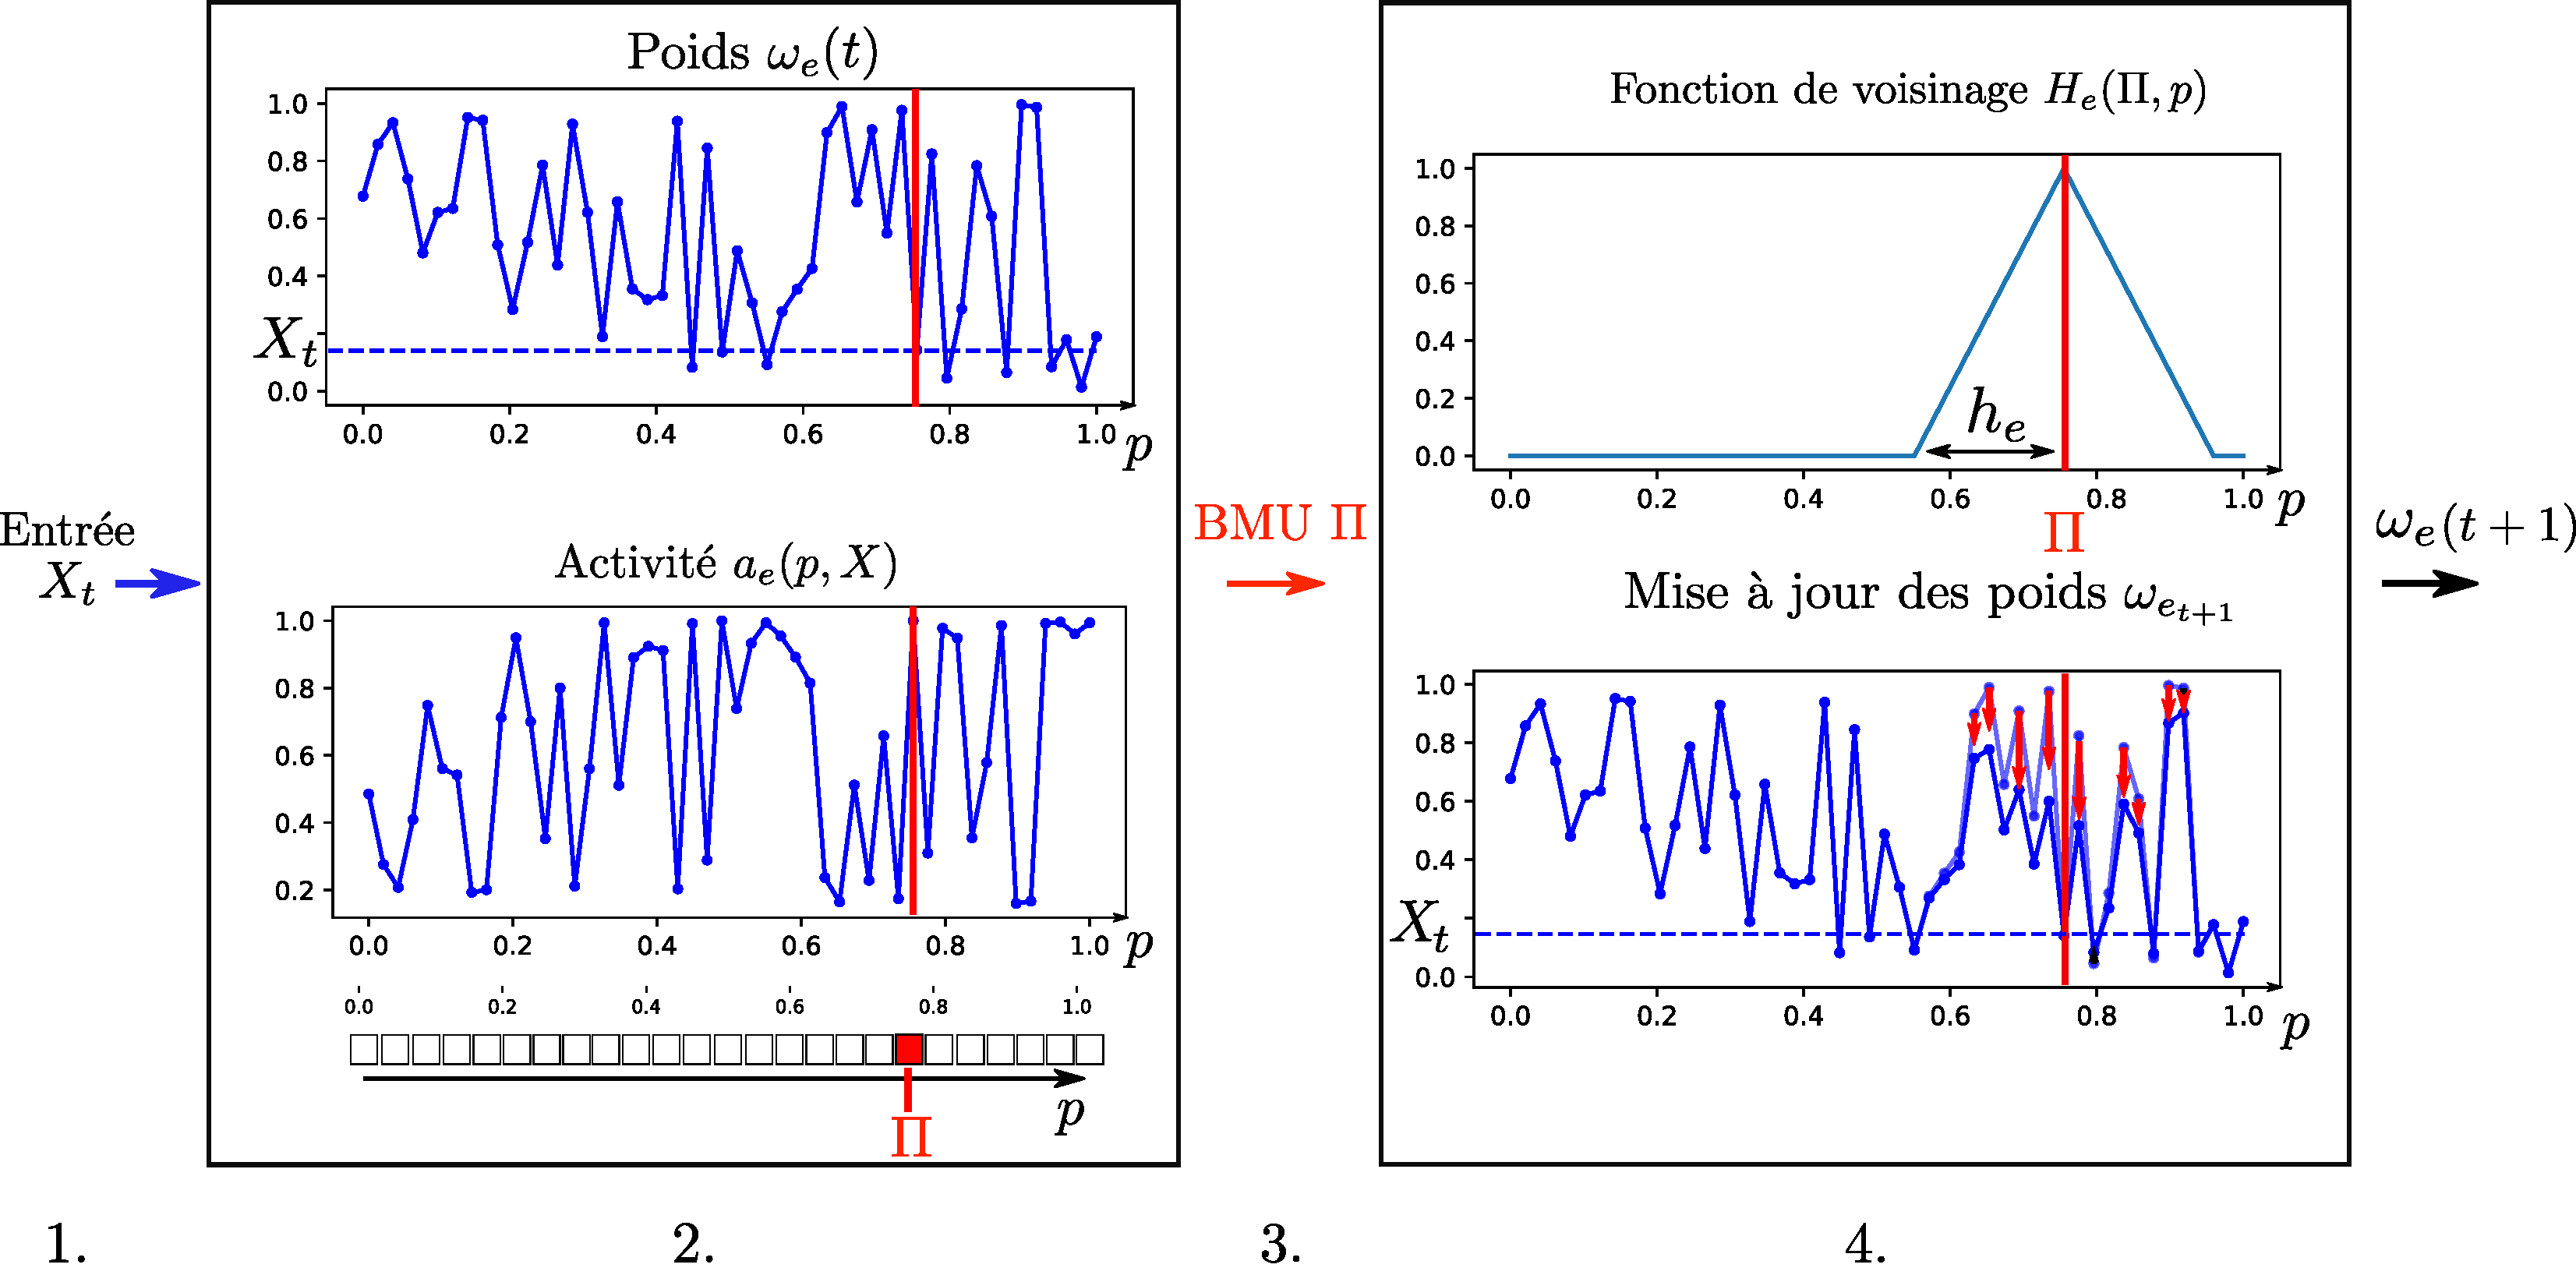
\includegraphics[width=\textwidth]{one_map_one_layer2.pdf}
\caption{Notations utilisées dans une carte de Kohonen simple. Les 4 étapes d'une itération d'apprentissage sont présentées: 1. Présentation de l'entrée, 2. Calcul de l'activité, 3. Choix du BMU, 4. Mise à jour des poids.}
\label{fig:one_map_not}
\end{figure}


\subsection{Paramètrage d'une carte de Kohonen}

L'organisation d'une carte de Kohonen est gérée par plusieurs paramètres. 
Nous détaillons ici les choix de paramètres effectués. 
Les paramètres supplémentaires introduits par la version CxSOM sont présentés en partie \ref{sec:params}.

\subsubsection{Taux d'apprentissage $\alpha$}

Le taux d'apprentissage $\alpha$ détermine la proportion dans laquelle chaque poids est déplacé vers l'entrée lors de sa mise à jour, selon l'équation~\ref{eq:update}. Dans l'algorithme classique, le taux d'apprentissage décroît au cours de l'apprentissage. Au début de l'apprentissage, $\alpha$ est élevé, ce qui assure un dépliement rapide de la carte. $\alpha$ est ensuite diminué manuellement tout au long de l'apprentissage. Cette décroissance accompagne la convergence des poids de la carte au cours de l'apprentissage.

Un objectif à long terme de développement de l'architecture CxSOM est de construire des systèmes de cartes autonomes dynamiques. Ces systèmes apprennent sur des données en ligne, présentées séquentiellement et ayant des dépendances temporelles. Dans ce cas d'utilisation, il n'est pas souhaitable de faire décroître le taux d'apprentissage qui introduit un début et une fin d'apprentissage fixés par avance. Le calcul d'une itération dépend alors non seulement de l'état précédent de la carte, mais aussi de l'itération $t$ courante. 
Nous choisissons ainsi de garder un $\alpha$ constant dans le modèle CxSOM.
Les calculs réalisés lors d'une itération $t$ dépendent alors uniquement de l'état de la carte au pas de temps précédent.

\subsubsection{Topologie de la carte}

Le graphe supportant la carte de Kohonen peut présenter diverses formes, comme détaillé en section~\ref{sec:som001}~: grilles, lignes, arbres, graphes \dots Les notations et l'algorithme CxSOM que nous présentons dans ce chapitre sont applicables à toutes les formes de cartes. Les expériences et l'évaluation du modèle se concentrent quant à elles sur des lignes 1D et des grilles 2D, et omettent les formes de graphes quelconques. Ce choix est d'abord motivé par le fait que les lignes et les grilles sont les formats de cartes les plus courants rencontrés dans la littérature. On parle souvent de cartes de Kohonen 1D et cartes 2D, en sous-entendant le format de ligne ou de grille du graphe support. 

Ensuite, la spécificité des cartes de Kohonen tient à l'organisation des prototypes de façon continue. Lorsqu'on parle de continuité des prototypes dans une carte de Kohonen, il s'agit d'abord d'une relation de proximité et d'ordre entre des prototypes discrets: \emph{si deux unités sont proches dans la carte, alors leurs prototypes sont proches dans l'espace d'entrée}. Un exemple d'organisation des poids d'une SOM en ligne 1D sur des données dans $[0,1]$ est tracé en figure~\ref{fig:depliement}. Les prototypes sont répartis aléatoirement dans l'espace d'entrée $[0,1]$ à l'itération $0$~; au cours de l'apprentissage, ils s'organisent de façon ordonnée. A partir de l'itération 500, on observe cette continuité des prototypes.

Le format particulier de ligne et de grille d'une carte de Kohonen permet d'étendre cette notion de proximité entre prototypes à une continuité des poids au sens mathématique, par interpolation. Dans ces formats 1D et 2D, l'ensemble des n\oe{}uds et leurs arêtes est inclus dans une ligne ou un plan~: chaque arête peut être vue comme un ensemble de positions. Les poids de la carte sont dans ce cas une approximation discrète d'une fonction continue $\widetilde{\w_e}$, à valeurs dans~$\mathcal{D}$.
\begin{equation*}
\begin{array}{ccccc}
M& : & [0,1]^2 \; \text{ou} \;[0,1] & \to &  \mathcal{D} \\
 & & p & \mapsto & \widetilde{\w_e}(p) \\
\end{array}
\end{equation*}

Cette continuité est une des puissances d'une carte de Kohonen en tant qu'algorithme de quantification vectorielle. 
% Des opérations réalisées dans l'espace des positions $[0,1]$ correspondent directement à des opérations dans l'espace d'entrée $\mathcal{D}$, par la fonction $\widetilde{\w_e}$.

Au cours de l'apprentissage, les poids d'une carte se rapprochent de la distribution des données. On parlera de \emph{dépliement} d'une carte lorsqu'on fait référence à son apprentissage.
Pour une carte 1D sur des données 1D, il est démontré en \cite{Kohonen1995SelfOrganizingM} que les poids évolueront au cours de l'apprentissage vers un ordre strictement croissant ou strictement décroissant~; ordre qui ne sera plus modifié une fois atteint. 
Lorsque la dimension des données est plus grande que celle de la carte, par exemple des points 2D ou des images, la carte formera des plis de manière à remplir l'espace $\mathcal{D}$ (voir figure~\ref{fig:som1d}, section~\ref{sec:som001}). 

\begin{figure}
\centering
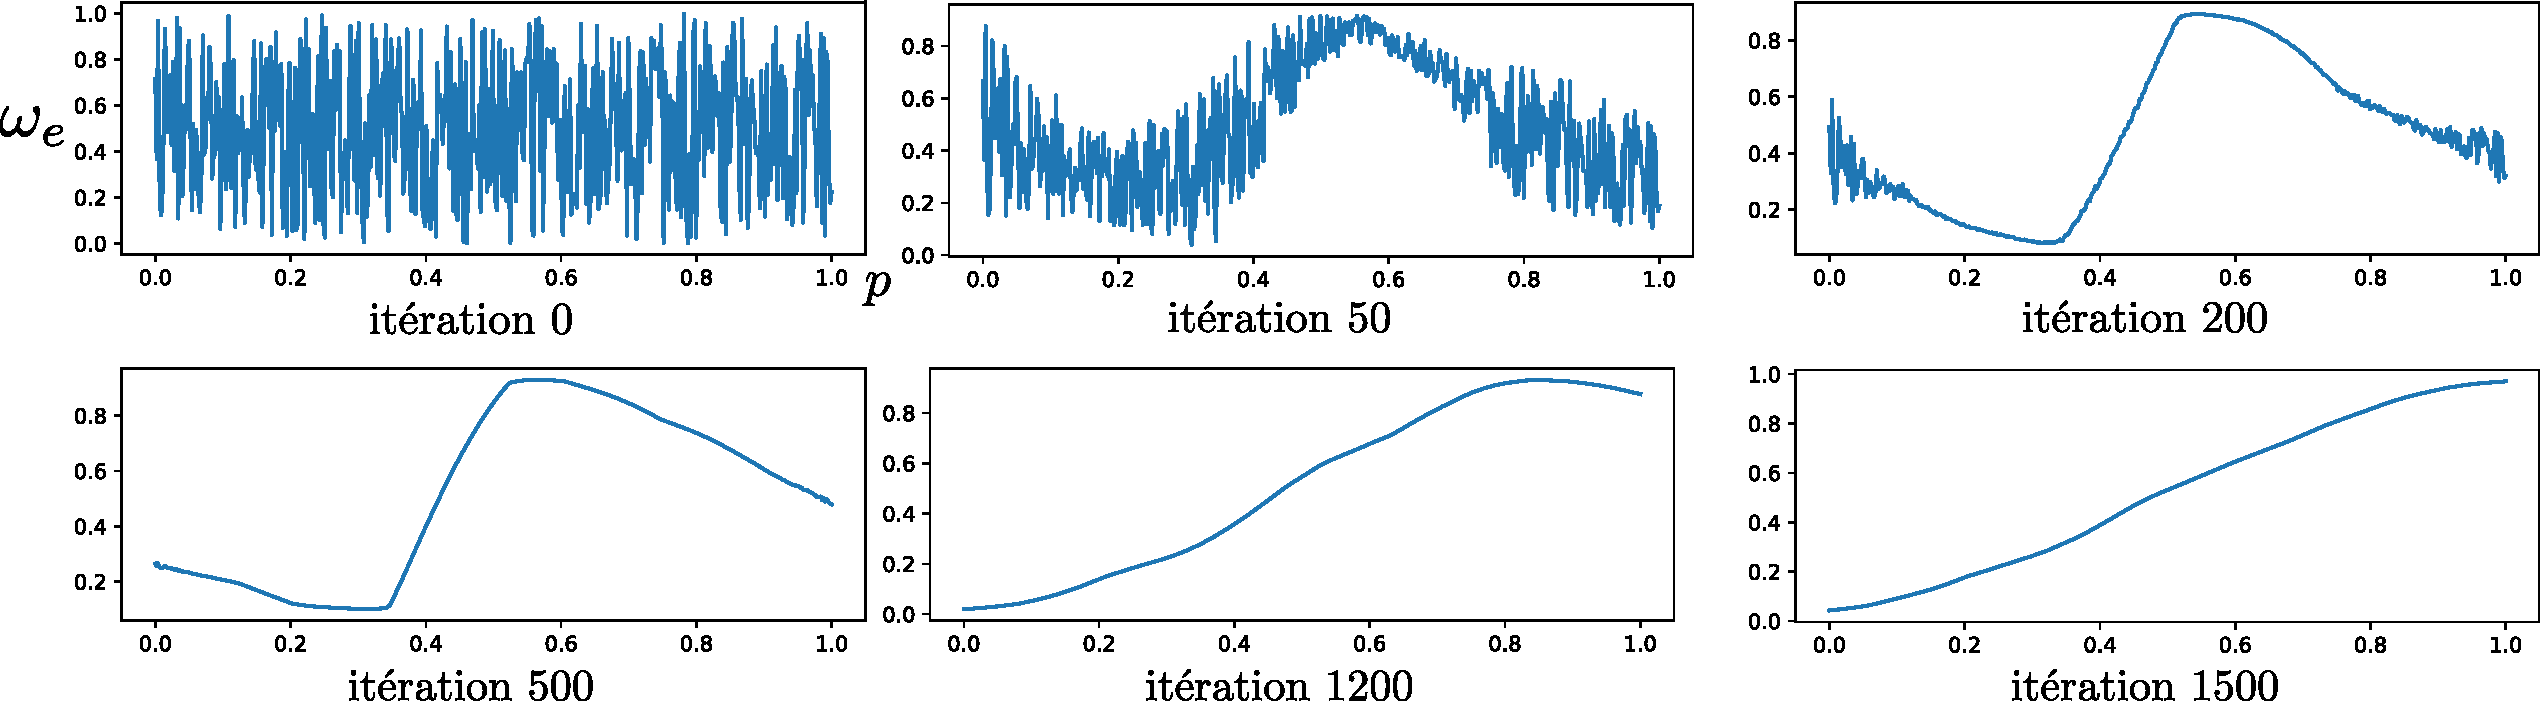
\includegraphics[width=\textwidth]{depliement_1D.pdf}
\caption{Exemple de dépliement d'une carte 1D de taille 500, sur des données 1D $\inpx \in [0,1]$. Les paramètres $h\ext = 0.2, \: \alpha = 0.2$ ont été gardés constants dans cet exemple. On s'attend à ce que les poids de la carte soient organisés selon un ordre strictement croissant ou décroissant à la fin de l'apprentissage.}
\label{fig:depliement}
\end{figure}

\subsubsection{Rayon de voisinage}

Le choix de la fonction de voisinage est déterminant dans la topologie de la carte. Elle dépend en particulier du rayon de voisinage $h_e$.
Cette valeur détermine quelles unités voisines du BMU auront leurs poids mis à jour.
Plus le rayon $h_e$ est grand, plus la partie de la carte dont les poids sont déplacés vers l'entrée lors de la mise à jour est étendue. 
Le rayon de voisinage détermine \emph{l'élasticité} d'une carte. 
Une carte ayant un grand rayon de voisinage est moins sensible aux variations locales des données et parvient à se déplier selon les variations à grande échelle de la distribution des entrées.
Un petit rayon d'apprentissage permet au contraire de déplacer les poids concentrés dans une petite région sans affecter toute la carte. Les poids s'ajustent ainsi aux variations locales des entrées. Par contre, choisir un rayon de voisinage petit dès le début de l'apprentissage empêche la carte de se déplier globalement de façon ordonnée; au contraire, on verra apparaître des portions distinctes de cartes s'organisant de façon discontinue.
Le choix de l'élasticité est donc un compromis entre apprentissage d'une structure globale des entrées et ajustement aux variations locales.
Dans l'algorithme classique, ce compromis est trouvé en faisant décroitre le rayon de voisinage au cours de l'apprentissage. Un grand rayon de voisinage permet à la carte de se déplier rapidement en apprenant une structure globale des données. Sa décroissance au cours des itérations permet d'affiner l'apprentissage des données à un niveau plus fin. 
Contrairement à la plupart des SOM classiques, nous garderons des rayons de voisinage constants dans CxSOM. Tout comme le fait de garder le taux d'apprentissage constant, garder le rayon de voisinage constant est motivé par les objectifs de traitement de données séquentielles, vers des systèmes de cartes utilisés en continu.

\section{Motivations du modèle CxSOM}
A partir du modèle de carte de Kohonen détaillé en section \ref{sec:kohonen}, nous proposons une version de carte auto-organisatrice servant de module de base pour construire des architectures non-hiérarchiques de cartes. 
L'idée de construire de telles architectures est d'apprendre plusieurs ensembles de données hétérogènes de façon jointe, et de réaliser également l'apprentissage des relations entre ces entrées.
Nous présentons tout d'abord les choix de développement effectués pour créer le modèle d'architecture.

\subsection{Champ d'application: mémoire associative}

La motivation à long terme d'une architecture de cartes est de construire des systèmes dynamiques apprenant sur un ensemble de capteurs en entrée, et pouvant traiter des données séquentielle.
Dans cette étude, nous nous concentrerons sur les capacités d'une architecture à apprendre des relations entre des entrées non temporelles. 
On considèrera un ensemble d'espaces $\mathcal{D}\m{1}, \cdots , \mathcal{D}\m{n}$ comme différentes \emph{modalités}.
Les entrées présentées à une architecture de cartes sont $(\inpx\m{1}_t, \cdots, \inpx\m{n}_t) \in \mathcal{D}\m{1} \times \cdots \times \mathcal{D}\m{n}$. On se place dans des cas où les distributions des modalités considérées $\inpx\m{i}$ dépendent les unes des autres. 
La tâche de mémoire associative consiste à extraire des schémas de dépendance entre ces modalités. 
Lorsqu'on tire une entrée pour la présenter à une carte, on tire une entrée jointe $\mathbf{\inpx} =  (\inpx\m{1}_t, \cdots , \inpx\m{n}_t)$, dont chaque composante est présentée à la carte qui lui correspond. 
Le but pour l'architecture de cartes est d'encoder une représentation de chaque espace d'entrée $\mathcal{D}\m{i}$ par quantification vectorielle et d'encoder le schéma de dépendances entre modalités au sein de l'architecture.

% Pour respecter l'homogénéité des entrées nécessaires à l'apprentissage d'une carte auto-organisatrice, nous normaliserons les espaces $\mathcal{D}\m{i}$ pour que toutes les entrées soient à valeur dans $[0,1]$ sur chaque dimension.
% Dans les exemples de cette thèse, nous tirerons des entrées jointes en deux ou trois dimensions, dont chaque composante 1D est présentée à une carte. Chaque modalité est la coordonnée sur un des axes du point 3D tiré. Nous utiliserons par exemple, en tant qu'espace dont les modalités sont dépendantes, un ensemble de points sur un cercle en une dimension dans un espace en trois dimensions. Chaque coordonnée $x$, $y$, $z$ dépend alors des deux autres coordonnées. Nous évaluerons comment l'architecture que nous présentons dans cette partie apprend les données ainsi que leurs relations. 

% Les exemples porteront sur des modalités en une dimension, mais les dimensions de chaque modalité peuvent être quelconque.

\begin{figure}
\centering
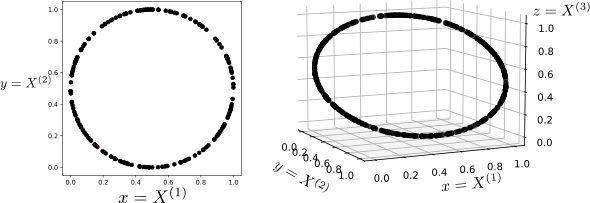
\includegraphics[width=\textwidth]{inputs_3som}
\caption{Exemple de disposition d'entrées en deux dimensions, à gauche, et trois dimensions, à droite. Les modalités associées à différentes cartes sont les coordonnées $x,y$ et $z$ de chaque point. Dans une telle disposition, les modalités dépendent les unes des autres~: développer une mémoire associative signifie apprendre le modèle de relation existant etre $x,y$ et $z$, c'est-à-dire le cercle.\label{fig:input_3som}}
\end{figure}

\subsection{Description de l'architecture}

Nous avons vu au chapitre précédent les possibilités d'interfaces entre cartes. 
Dans CxSOM, on choisit de se placer dans le paradigme de transmission de la position du BMU entre cartes: on connecte une carte B à une carte A en donnant la position du BMU de B en entrée à la carte A. 
% Ce paradigme de partage de positions rappelle à la fois le modèle hiérarchique HSOM~\cite{lampinen_clustering_1992}, et les modèles de cartes récurrentes s'appuyant sur SOMSD \cite{hammer_recursive_2004,hagenbuchner_self-organizing_2003,fix20}. 
Contrairement aux cartes hiérarchiques comme HSOM~\cite{lampinen_clustering_1992} dans lesquelles la position du BMU est la seule entrée d'une carte de plus haut niveau, chaque carte de l'architecture peut posséder une entrée principale propre issue d'une modalité $\inpx\m{i}$ que nous appelons l'entrée \emph{externe}. 
Une carte prendra ensuite un ensemble d'entrées secondaires qui sont les positions des BMUs des autres cartes de l'architecture. 
Les cartes auto-organisatrices dans le modèle CxSOM prennent donc un nombre arbitraire d'entrées, dont certaines sont les BMUs d'autres cartes. On appelle ces entrées internes à l'architecture les entrées \emph{contextuelles} d'une carte.
L'algorithme d'apprentissage d'une carte auto-organisatrice prenant une position de BMU en tant que contexte est similaire à celui d'une carte classique, comprenant:
\begin{enumerate}
\item\label{etape:entree} Présentation des entrées externes et contextuelles à chaque carte 
\item\label{etape:bmu} Recherche du BMU par calcul d'activité
\item\label{etape:maj} Mise à jour des poids selon une fonction de voisinage
\end{enumerate}
Chaque carte aura simplement plusieurs entrées: une entrée \emph{externe} dans un espace d'entrée, et $k$ entrées \emph{contextuelles} qui sont les positions des BMUs des cartes qui lui sont connectées. 
Une carte peut aussi ne pas prendre d'entrée externe, seulement des entrées contextuelles.

Toutefois, la recherche du BMU doit être modifiée par rapport à la méthode originale~: les rétroactions entre les cartes étant autorisées, la position du BMU de la carte A va donc influencer la position du BMU de la carte B, laquelle modifie à nouveau le BMU de la carte A, etc. 

Notre algorithme implémentera deux modifications principales par rapport à l'algorithme d'apprentissage d'une carte de Kohonen classique: 
\begin{itemize}
\item Les cartes possèdent plusieurs entrées, externes et contextuelles; les entrées contextuelles sont les positions des BMUs d'autres cartes. Le calcul de l'activité est modifié afin de prendre en compte ces différentes couches d'entrées.
\item La recherche du BMU est modifiée afin de gérer les rétroactions entre cartes.
\end{itemize}

L'architecture CxSOM couple ainsi l'apprentissage de plusieurs cartes. Elles apprennent à la fois sur leurs données $\inpx\m{i}$, mais contextualisées selon les informations issues des autres cartes. Notons que les cartes apprennent de façon jointe dès le début de leur apprentissage. 

Seule la position du BMU est utilisée comme information transmise entre carte. Cette valeur a l'avantage d'apporter une homogénéité dans l'architecture de cartes~: quelles que soient les entrées d'une carte et leurs dimensions, le BMU sera une position en 1 ou 2 dimensions. Si on prenait le poids du BMU comme valeur transmise, par exemple, comme peut le faire la carte récurrente MSOM~\cite{Strickert2005MergeSF}, l'information circulant entre les cartes dépendrait des dimensions des entrées.
De plus, transmettre seulement la position du BMU est une avantage en terme de quantité d'information à transmettre: il s'agit d'un vecteur en une ou deux dimension.
La transmission de cette position, on le verra dans le chapitre d'analyse, est suffisante pour permettre un apprentissage du modèle de relations entre données.
On laisse aussi la possibilité d'utiliser des cartes ne prenant que des entrées contextuelles. Ces cartes agissent alors comme des cartes intermédaires, connectant des cartes prenant des entrées externes.

L'algorithme CxSOM est détaillé en algorithme~\ref{algo:cxsom}; les parties suivantes expliquent et illustrent le modèle. Nous présentons d'abord le modèle sur un exemple d'une architecture de deux cartes, puis nous présentons l'algorithme formalisé dans un cadre général d'architecture.

\section{Présentation de CxSOM: exemple d'une architecture de deux cartes}

Avant de présenter le modèle général de CxSOM sur une architecture quelconque, présentons le fonctionnement de l'architecture la plus simple qui soit~: deux cartes $M\m{1}$ et $M\m{2}$, connectées réciproquement, présentée en figure~\ref{fig:2som_archi}. Toutes les équations seront ensuite formalisées dans le cas général en section~\ref{sec:formalisme}. 
Nous prenons dans cet exemple des cartes en une dimension, indexées par $p \in [0,1]$.

\subsection{Détail des étapes}


\paragraph{Structure d'une carte}

Chaque carte $M$ de l'architecture prend une entrée externe, $\inpx$ et une entrée contextuelle $\inpc$ qui est la position courante du BMU de l'autre carte.
Les entrées externes $\inpx\m{1}_t$ et $\inpx\m{2}_t$ sont deux modalités interdépendantes.
On indicera les élements des cartes par $(1)$ et $(2)$ pour désigner les éléments appartenant à la carte $M\m{1}$ et $M\m{2}$.
Une carte $i$ ($i \in {1,2}$) possède deux couches de poids afin de traiter les deux entrées~: les poids \emph{externes} $\w_e\m{i}$,  qui se déplient sur les entrées $\inpx\m{i}$, et les poids contextuels $w_c\m{i}$, qui se déplient sur les entrées contextuelles, qui appartiennent à l'espace des positions en une dimension de l'autre carte. 
Ces deux couches de poids sont représentées en figure~\ref{fig:2som_weights}. La position du BMU de $M\m{2}$, $\bmu\m{2}_t$ est utilisée comme entrée contextuelle de $M\m{1}$, et $\bmu\m{1}_t$ comme entrée contextuelle de $M\m{2}$. 
Les deux cartes apprennent donc de façon couplée.

\paragraph{Calcul d'activité}

Chaque carte calcule une activité sur chaque entrée externe et contextuelle et les combinent en une activité globale permettant de calculer un BMU commun à toutes les couches de poids de la carte.
Les activités externes et contextuelles sont calculées comme dans le modèle classique, équation~\ref{eq:act1som} et tracées en figure~\ref{fig:2som_activite}.
Pour la carte $M\m{1}$, au pas de temps $t$, on a ainsi~:
\begin{equation}
\label{eq:activite}
\begin{cases}
a_e\m{1}(\inpx_t\m{1},p) = \exp\frac{-\lVert \w_e\m{1}(p)-\inpx\m{1}_t \rVert^2}{2\sigma^2} \\
a_c\m{1}(\bmu\m{2}_t,p) = \exp\frac{-\lVert \w_c\m{1}(p)-\inpc\m{1}_t \rVert ^2}{2\sigma^2}\\
\end{cases}
\end{equation}

$a_c$ et $a_e$ sont ensuites combinées en une activité globale définie de la façon suivante~:
\begin{equation}
a_g\m{1}(\inpx\m{1},\inpc\m{1}_t,p) = \sqrt{a_e(\inpx_t,p)\times \frac{a_e(\inpx_t,p) + a_c(\inpc\m{1}_t,p)}{2}}
\end{equation}
Par la différence de contribution de $a_c$ et $a_e$ au sein de l'activité globale -- $a_c$ ne contribue qu'à la puissance $\frac{1}{2}$ -- on assure que l'activité contextuelle vient seulement moduler l'activité externe.
On peut observer cette modulation sur la courbe noire de la figure~\ref{fig:2som_activite}~: l'activité globale suit la même progression que l'activité externe, mais est modifiée localement par les variations de l'activité contextuelle. 
De cette façon, les entrées contextuelles ne viennent pas donner d'\og hallucinations \fg{} à la carte~: elle apprend en priorité ses entrées externes, conditionnées aux entrées contextuelles. Ce choix de combinaison d'activité est issu du modèle de cartes cellulaires Bijama développé au sein de notre équipe \cite{menard05,khouzam_2013}.

\begin{figure}
\centering
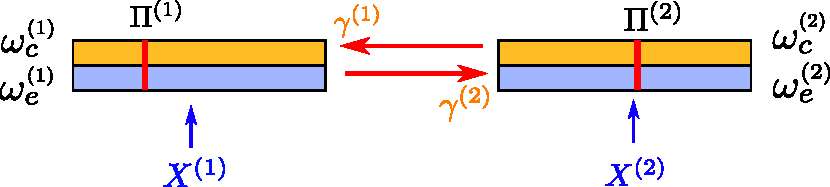
\includegraphics[width=0.7\textwidth]{archi_2som}
\caption{Architecture la plus simple possible de deux cartes. Le BMU $\bmu\m{1}_t$ de la carte $M\m{1}$ est utilisé en entrée contextuelle de $M\m{2}$, et le BMU $\bmu\m{2}_t$ de $M\m{2}$ en entrée contextuelle de $M\m{1}$. Chaque carte possède donc deux couches de poids.
\label{fig:2som_archi}}
\end{figure}

\begin{figure}
\centering
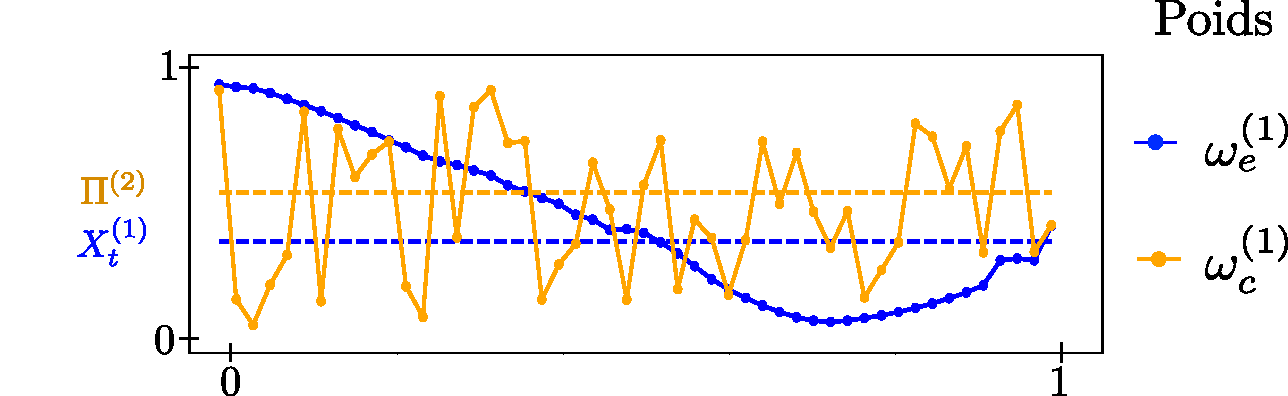
\includegraphics[width=0.75\textwidth]{weights_2som.pdf}
\caption{Représentation des poids de $M\m{1}$. L'entrée externe $\inpx_t$ présentée à l'itération $t$, tirée d'un espace d'entrée 1D $[0,1]$, est indiquée en bleu sur le graphique. L'entrée contextuelle $\inpc$ est le BMU de la carte $M\m{2}$. Sa valeur est indiquée en jaune; il s'agit d'une position 1D dans la carte $M\m{2}$, à valeur entre 0 et 1. La configuration des poids présentée dans cet exemple est atteinte durant le processus d'apprentissage de deux cartes $M\m{1}$ et $M\m{2}$, dont les entrées $\inpx\m{1}_t$ et $\inpx\m{2}_t$ sont les coordonnées de points tirés sur un cercle. \label{fig:2som_weights}}
\end{figure}

\paragraph{Relaxation}

Le calcul de $\bmu\m{1}_t$ dépend donc de $\bmu\m{2}_t$ et inversement. Contrairement à une carte simple, on ne peut pas calculer tous les BMUs de l'architecture un par un en prenant $\hat{p}$, l'argmax de $a_g$, comme BMU dans chaque carte.
On remplace l'étape de simple calcul d'argmax par un processus global à l'architecture de recherche de BMU. Cette recherche est réalisée par un processus dynamique que l'on appelera \emph{relaxation}, menant à un \emph{consensus} entre cartes~: on cherche un point, s'il existe, où le BMU dans chaque carte est au plus proche du maximum de son activité globale $\hat{p}$.

Cette recherche est réalisée par une sous-boucle incluse dans un pas d'apprentissage $t$, indexée par $\tau$. Cette sous-boucle définit une suite de positions intermédaires, $(\bmu\m{1}_\tau , \bmu\m{2}_\tau)$, permettant de chercher le BMU itérativement.
Le processus de relaxation est le suivant~:
\begin{enumerate}
\item Les entrées externes sont présentées au début de la boucle, donc $a_e$ peut être calculée; $\bmu\m{1}_0$ et $\bmu\m{2}_0$ sont initialisées à la position où les activités externes sont maximales dans chaque carte. 
\item Tant que la suite de positions $(\bmu\m{1}_\tau,\bmu\m{2}_\tau)$ n'a pas convergé:
	\begin{enumerate}
	\item Dans chaque carte, nous calculons les activités contextuelles et globales, définissant ainsi $\hat{p}\m{1}_\tau = \argmax_p(a_g\m{1}(p,\inpx\m{1}, \bmu\m{2}_\tau)$, de même pour $\hat{p}\m{2}$.
	\item Nous déplaçons $\bmu\m{1}$ vers $\hat{p}\m{1}$ et $\bmu\m{2}_\tau$ vers $\hat{p}\m{2}$ d'un pas $\Delta$: $\bmu\m{1}_{\tau+1} = \bmu\m{1}_{\tau} \pm \Delta$.
	Si une des valeurs est plus proche de $\hat{p}$ que $\Delta$, on déplacera $\bmu_\tau$ directement sur $\hat{p}$ pour éviter les oscillations autour du point. Cette étape est illustrée en figure~\ref{fig:relax}.
	\end{enumerate}
\item Le BMU de chaque carte est pris comme la valeur finale stable de ce processus dynamique.
 On note cette position finale $\bmu\m{i}_t$. Cette valeur sera celle utilisée dans chaque carte pour les mises à jour des poids.
 Si la relaxation n'atteint pas de point stable, nous fixons tout de même un nombre d'itérations maximum $\tau_{max}$ après lequel on arrête la relaxation.
\end{enumerate}

\paragraph{Mise à jour}

Enfin, chaque couche de poids $\w\ext\m{i}$, $\w_c\m{i}$ est mise à jour indépendamment dans chaque carte relativement au BMU $\bmu\m{i}_t$ et aux entrées externes $\inpx\m{i}_t$ et contextuelles $\bmu\m{j}_t$. Cette mise à jour correspond à la figure~\ref{fig:maj}. 
Notons que nous choisissons des rayons d'apprentissage sont différents entre couche externe et couche contextuelle~; nous détaillerons ce choix au cours des expériences.

\begin{figure}
\centering
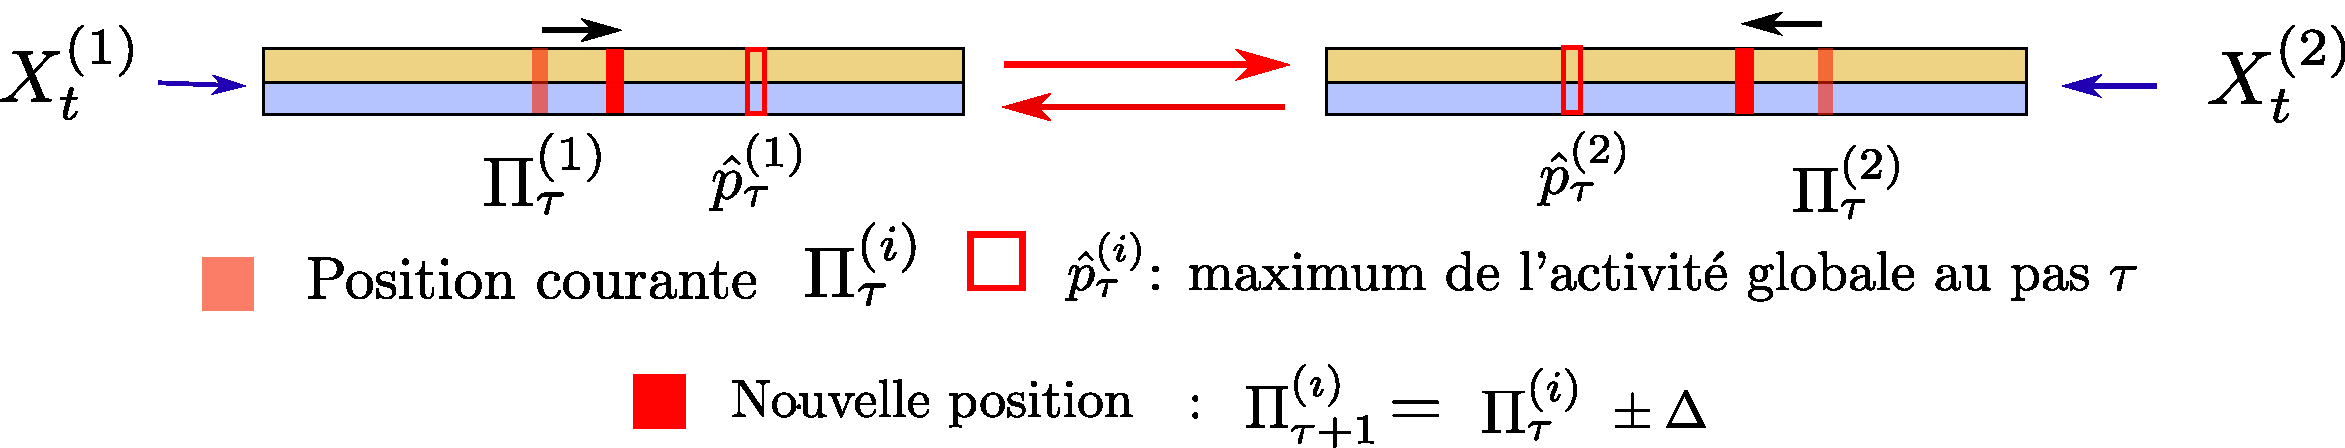
\includegraphics[width=\textwidth]{relaxation_2maps.pdf}
\caption{Description d'une étape de relaxation dans l'architecture, aboutissant à un consensus entre cartes. Lors de la relaxation, les positions $\bmu_\tau$ sont légèrement déplacées jusqu'à ce que toutes les positions $\bmu_\tau$ des cartes de l'architecture soient stables. Ce point de convergence correspond à un ensemble de positions qui maximise l'activité de chaque carte. \label{fig:relax}}
\end{figure}

\begin{figure}
%\begin{minipage}{0.6\textwidth}
\centering
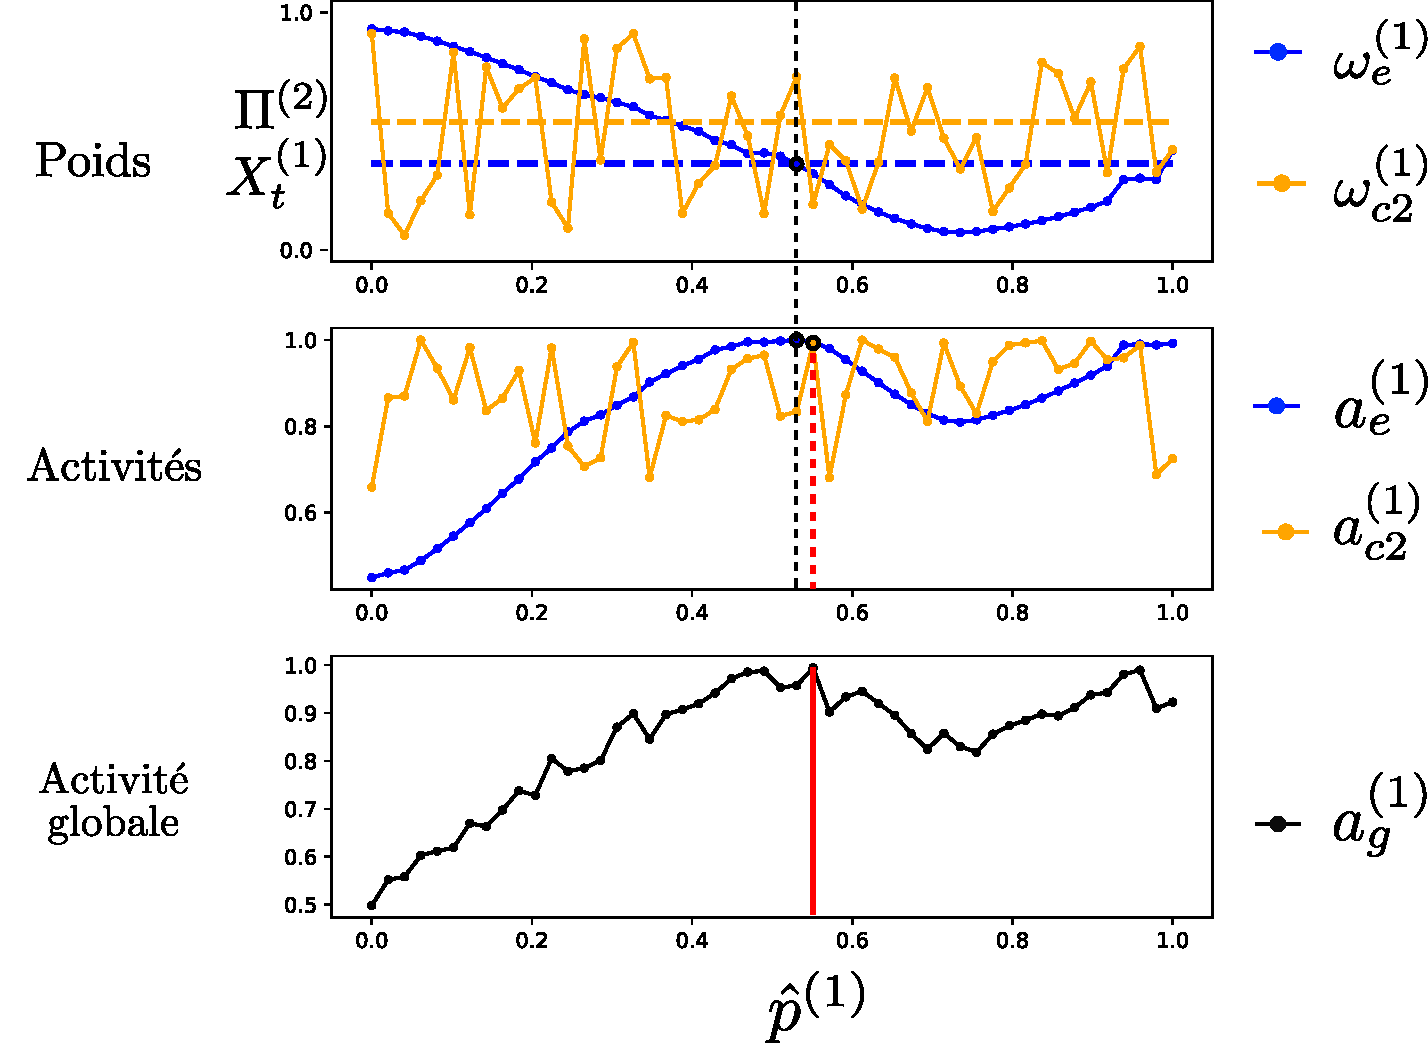
\includegraphics[width=0.8\textwidth]{activite_layers_2maps.pdf}
%\end{minipage}
%\begin{minipage}{0.35\textwidth}
\caption{Calcul d'activité dans une SOM au sein d'une architecture de deux cartes. La carte prend une entrée externe et une entrée contextuelle. 
L'indice $(1)$ permet de distinguer les éléments relatifs à cette carte. 
L'entrée externe est $X\m{1}_t$. La carte possède deux couches de poids, permettant de calculer deux activités. L'activité globale prend en compte tout les couches d'activités afin de trouver un BMU commun pour toutes les couches de poids. Le calcul de l'activité globale favorise l'activité externe et est modulé par l'activité contextuelle, ce qu'on observe sur la courbe du bas~: l'activité globale suit les variations de l'activité externe, et est localement modifiée par les variations de l'activité contextuelle.
Le maximum de l'activité globale est noté $\hat{p}$. \`A partir de l'activité globale, le BMU $\bmu\m{1}_t$ sera trouvé par le processus de relaxation décrit en partie~\ref{sec:relax}\label{fig:2som_activite}}
%\end{minipage}
\end{figure}

\begin{figure}
\centering
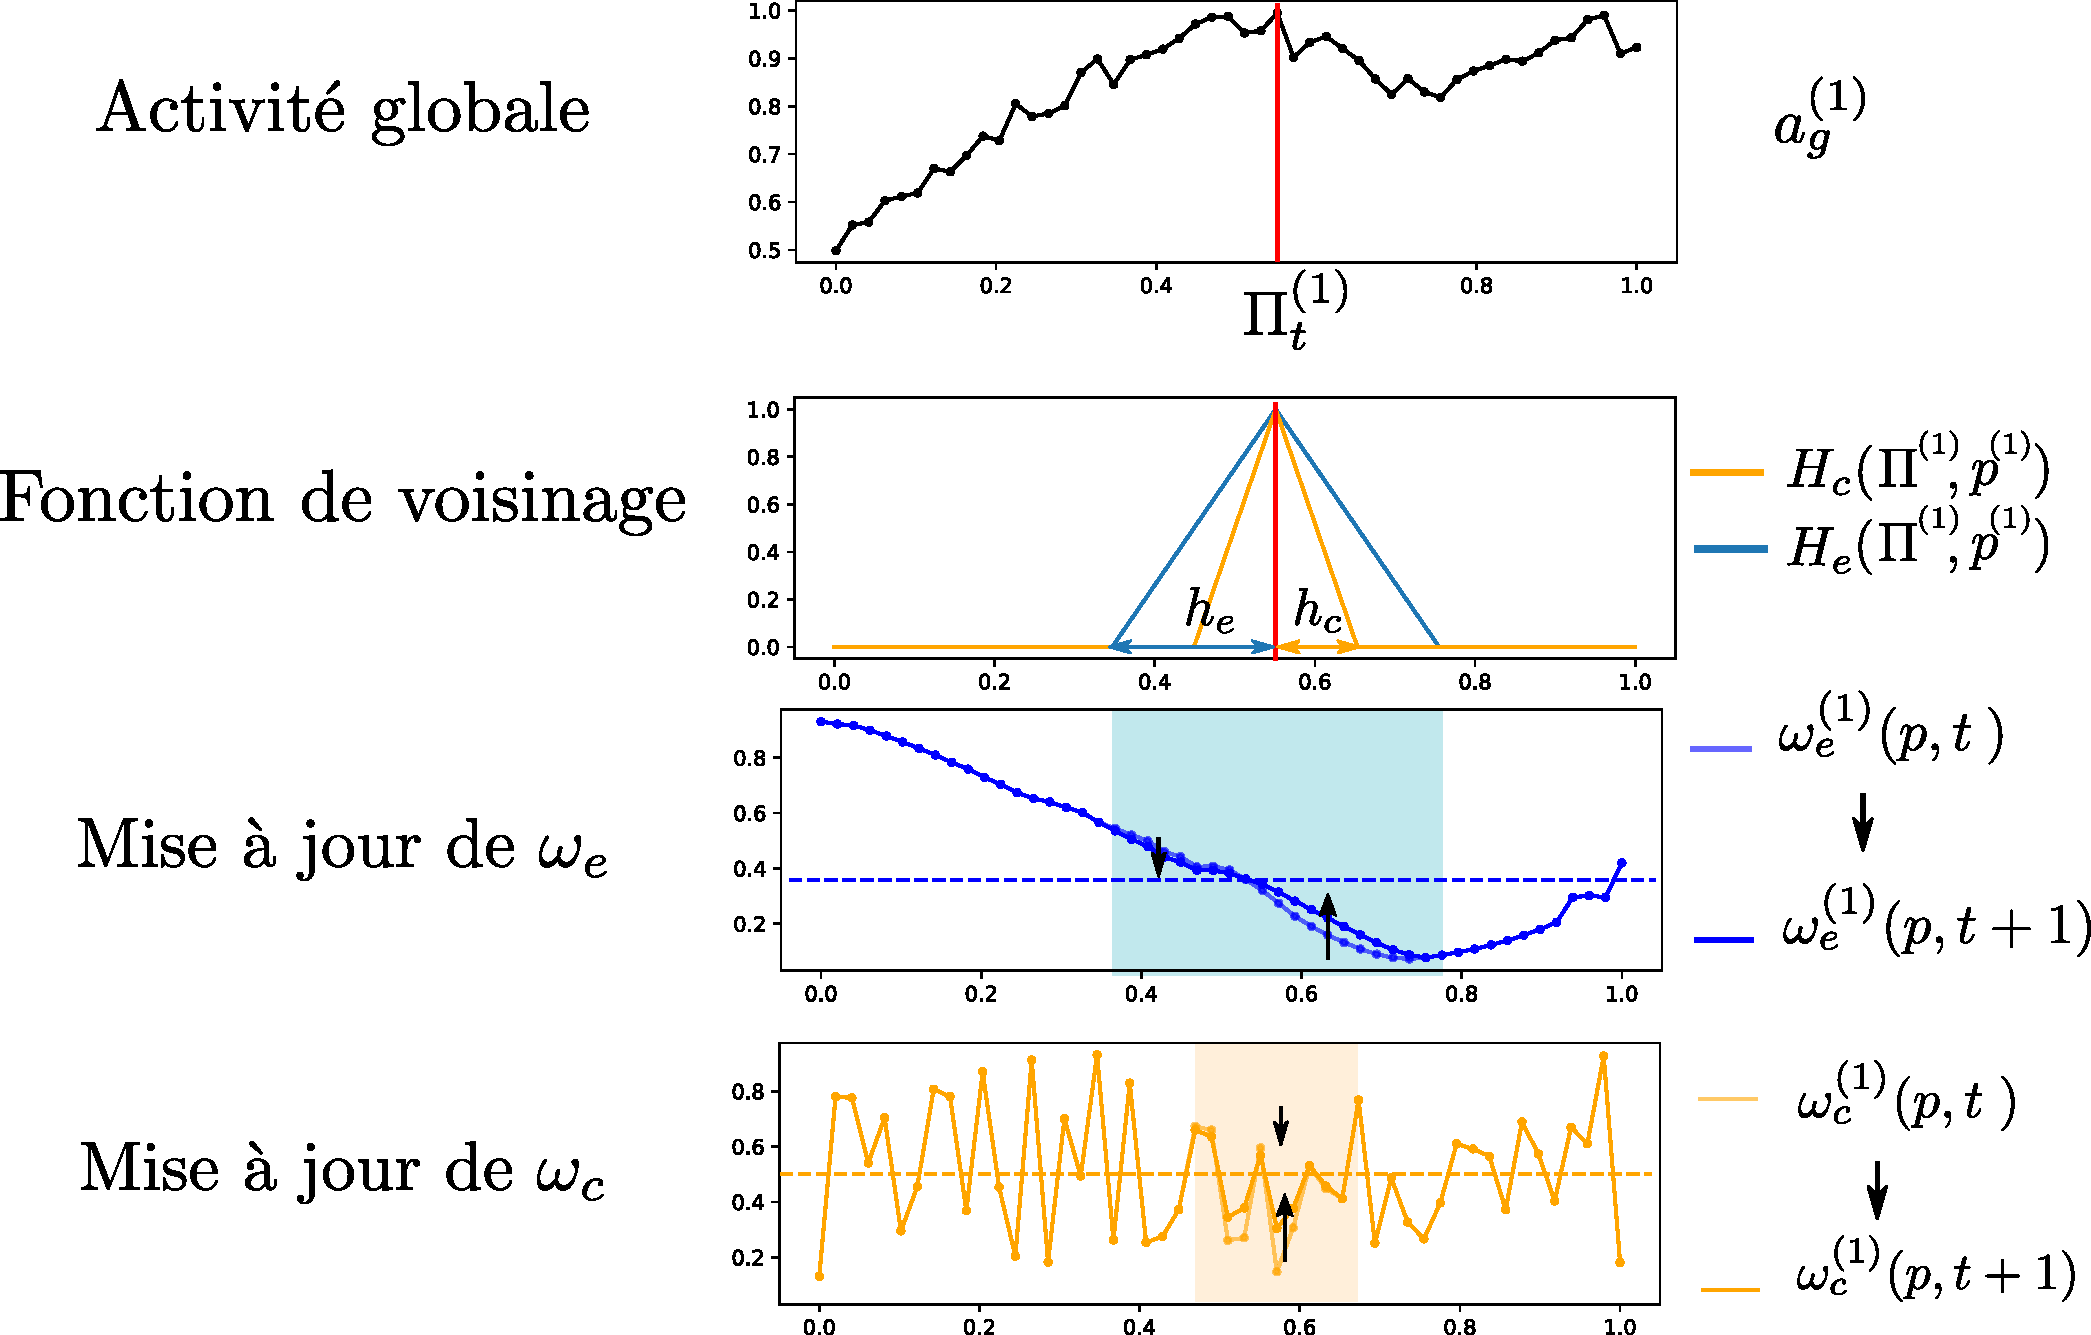
\includegraphics[width=0.9\textwidth]{maj_2som.pdf}
%\end{minipage}
%\begin{minipage}[c]{0.35\textwidth}
\caption{Mise à jour de chaque couche de poids indépendamment, relativement au BMU commun $\bmu\m{1}_t$, calculé par relaxation. Si la relaxation a convergé, la position $\bmu\m{1}_t$ est à la position $\hat{p}\m{1}$ maximisant l'activité globale à la fin de la relaxation. Le rayon de voisinage $h_e$ est utilisé pour mettre à jour les poids externes, le rayon $h_c$ pour mettre à jour les poids contextuels. On choisit $h_e > h_c$. Cette différence permet une différence de rythme d'apprentissage entre couches de poids. 
Ce choix sera expliqué dans les chapitres suivants.\label{fig:maj}}
%\end{minipage}
\end{figure}

\subsection{Résumé}
Les étapes d'un pas d'apprentissage $t$ d'une architecture de deux cartes sont les suivantes~; elles sont schématisées en figure~\ref{fig:algo}.
\begin{enumerate}
\item Présentation des entrées $\inpx\m{1}_t$ et $\inpx\m{2}_t$ à chaque carte
\item Relaxation~:
\begin{enumerate}
\item Calcul de l'activité externe $a_e(p, \inpx\m{i})$ dans chaque carte et initialisation des BMUs $(\bmu\m{1}_0,\bmu\m{2}_0)$ pour la relaxation.
\item Relaxation par petits déplacements de ($\bmu\m{1}_\tau,\bmu\m{2}_\tau$) dans chaque carte, avec calcul de l'activité contextuelle et globale à chaque pas $\tau$, jusqu'à une stabilisation du couple de valeurs $(\bmu\m{1}_\tau,\bmu\m{2}_\tau)$
\item Définition des positions des BMU $\bmu\m{1}_t,\bmu\m{2}_t$ comme la valeur de $(\bmu\m{1}_\tau,\bmu\m{2}_\tau)$ à l'issue de la relaxation.
\end{enumerate}
\item Mise à jour des poids $\w\ext\m{i}$ et $\w\cont\m{i}$ dans chaque carte, selon sa position du BMU $\bmu\m{i}_t$, son entrée externe $\inpx\m{i}_t$ et son entrée contextuelle $ \inpc\m{i} = \bmu\m{j}_t$, avec $\bmu\m{j}_t$ la position du BMU calculée par relaxation dans l'autre carte.
\end{enumerate}

\begin{figure}
\centering
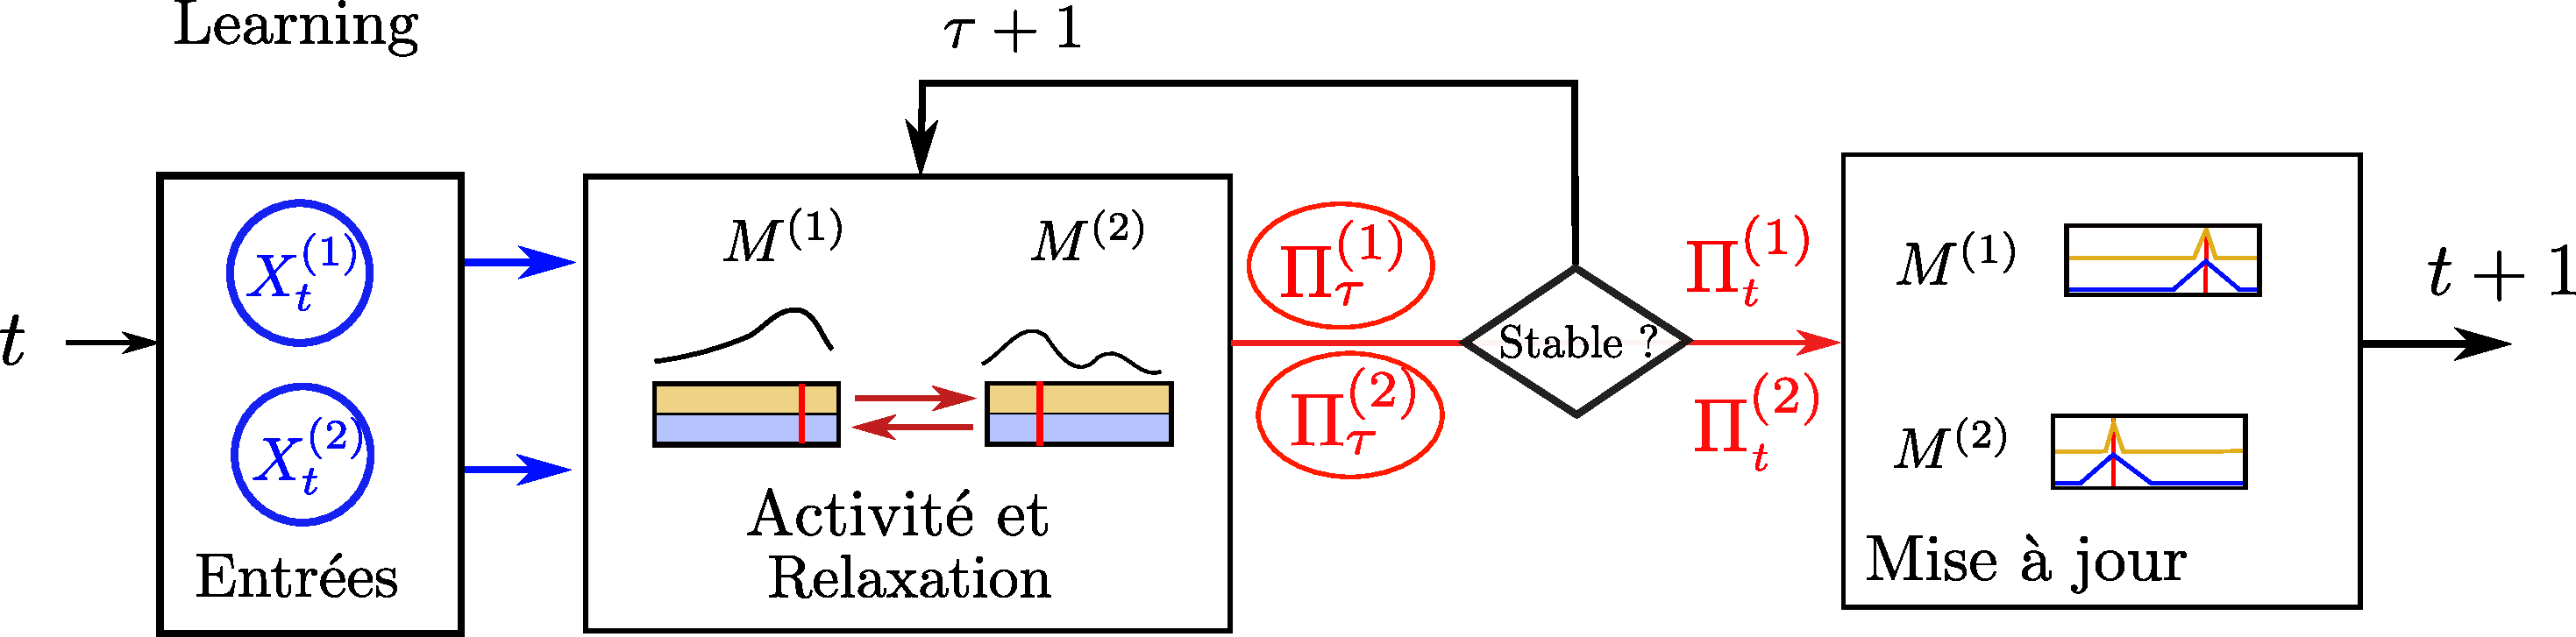
\includegraphics[width=\textwidth]{learning_tests_2maps}
\caption{Résumé des étapes de l'algorithme d'apprentissage d'une architecture, composé d'une boucle de recherche de BMU par relaxation dans laquelle les cartes sont couplées, puis d'une étape de mise à jour des différentes couches de poids séparément sur chaque carte.}
\label{fig:algo}
\end{figure}

\section{Formalisation: cas pour $n$ cartes}\label{sec:formalisme}

Nous présentons dans cette partie l'algorithme général pour une architecture quelconque de $n$ cartes. 
Les notations sont valables pour des cartes de dimension quelconque~; les entrées que nous avions illustrées par des valeurs 1D sont également de dimension quelconque.
La différence principale avec l'exemple à deux cartes est qu'une carte peut prendre plusieurs entrées contextuelles, qui sont les BMUs de toutes les cartes qui lui sont connectées dans l'architecture, au lieu d'une seule dans le cas de l'exemple à deux cartes. On retrouvera donc les notations de la partie précédente.
Cette partie concentre toutes les notations et l'algorithme utilisé dans cette thèse. 
L'algorithme est résumé en algorithme~\ref{algo:cxsom}.

\subsection{Entrées et calcul d'activité}

Dans une architecture composée de $n$ cartes, les cartes sont indexées par $i \in \{1,\cdots,n\}$. On indicera chaque élément d'une carte $M\m{i}$ par l'exposant $(i)$.
Pour faciliter la lecture, nous omettrons l'exposant $(i)$ dans les équations, lorsqu'on se concentre sur une seule carte. $\inpx_t$ désigne donc $\inpx_t\m{i}$, $\w_e$ désigne $\w_e\m{i}$, etc.

Lors d'un pas d'apprentissage $t$, une carte $M\m{i}$ reçoit en entrée une entrée \emph{externe} notée $\inpx_t$ et $K$ entrées \emph{contextuelles}. Notons-les pour le moment $\Gamma = (\inpc_1},\cdots,\inpc_K)$; elles seront les positions du BMU $\bmu\m{i_k}$ des cartes d'indice $k$ qui lui sont connectées~: $\bmu\m{i_k}_\tau$ lors de la relaxation puis $\bmu\m{i_k}_t$ lors de la mise à jour. La gestion des entrées contextuelles sera décrite avec le processus de relaxation en section suivante~; notons pour le moment que les entrées contextuelles sont des positions 1D ou 2D dans des cartes. 

La carte possède donc $K+1$ couches de poids. On  note $\w_e(p)$ les poids externes et $\w_{ci_1}(p), \cdots, \w_{ci_K}(p)$ les poids correspondant aux entrées contextuelles, les \emph{poids contextuels}.
$\w_{ci_k}$ correspond à la couche de poids relative à l'entrée contextuelle $\inpc_{i_k}$. Les poids externes sont à valeur dans $\mathcal{D}\m{i}$, la modalité associée à la carte $i$. Les poids contextuels sont à valeur dans l'espace des positions d'une cartes, soit $[0,1]$ en 1D ou $[0,1]^2$ en 2D.

Les activités externes et contextuelles s'expriment de la façon suivante:
\begin{equation}
\label{eq:activite_general}
\begin{cases}
a_e(\inpx_t,p) = \exp\frac{-\lVert \w_e(p)-\inpx_t \rVert^2}{2\sigma^2} \\
a_{ck}(\inpc_{i_k},p) = \exp\frac{-\lVert \w_{ci_k}(p)-\inpc_{i_k} \rVert ^2}{2\sigma^2}, \\
\text{Avec $i_k$ les indices des cartes connectées à $i$}
\end{cases}
\end{equation}

Notons $a_c(p, \Gamma)$ la moyenne des activités contextuelles, avec $\Gamma = (\inpc_{i_1}, \cdots, \inpc_{i_K})$.
\begin{equation}\label{eq:ac}
a_c(p, \Gamma) = \frac{1}{K}\sum_{k=1}^K {a_{ci_k}(p,\inpc_{i_k})}
\end{equation}

L'activité globale $a_g$ est calculée en combinant l'activité externe et la moyenne des activités contextuelles:
\begin{equation}
\label{eq:global_act}
a_g(\inpx_t,\Gamma,p) = \sqrt{a_e(p, \inpx_t) \frac{a_e(p, \inpx_t) +  a_c(p, \Gamma)}{2}}
\end{equation}

On notera également $\hat{p}$ la position du maximum de l'activité globale~:
\begin{equation}
\label{argmax}
\hat{p} = \argmax_p a_g(p, \inpx_t, \Gamma,)
\end{equation}

Notons qu'une carte peut ne pas avoir d'entrée externe. Dans ce cas, on prendra comme activité globale $a_c$, la moyenne des activités contextuelles (équation~\ref{eq:ac}).

\subsection{Calcul du BMU par relaxation}\label{sec:relax}

Dans chaque carte $i$, l'entrée contextuelle $\inpc\m{i}_{i_k}$ est le BMU à l'instant courant $\bmu\m{i_k}_t$  de la carte $k$. La position $\bmu\m{i}_t$ dépend donc des BMUs des autres cartes, qui dépendent eux-mêmes de $\bmu\m{i}_t$.
On cherche un ensemble de positions $\mathbf{\bmu}_t = (\bmu\m{1}_t, \cdots, \bmu\m{n}_t)$, si elles existent, telles que dans chaque carte, $\bmu\m{i}_t$ correspondent la position du maximum de l'activité globale, c'est-à-dire $\hat{p}\m{i}$.

\begin{equation}
\forall i, \; \bmu\m{i}_t = \argmax_{p} a_g\m{i}(p, \inpx\m{i}_t, \inpc_0, \cdots, \inpc_K)
\end{equation}

Le processus de relaxation est une boucle imbriquée dans un pas d'apprentissage de l'architecture, indexée par $\tau$. Dans chaque carte, on construit une suite de positions $\bmu\m{i}_\tau$, dont la valeur finale sera le BMU $\bmu\m{i}_t$.

Lors d'une itération $t$, chaque carte est nourrie avec une entrée externe $\inpx\m{i}_t$ qui restera constante au cours de la relaxation. 
Les activités externes $a_e\m{i}(p, \inpx\m{i}_t)$ de chaque carte peuvent être calculées dès le début de la relaxation.
La relaxation est définie comme suit~:
\begin{enumerate}
\item Dans chaque carte $i$, la position $\bmu\m{i}_0$ est initialisée à $\hat{p}\m{i}_0 = \argmax_{p\m{i}}(a_e\m{i}(\inpx\m{i}_t,p)$.
\item Dans chaque carte $i$, on assigne $\inpc_{i_k}\m{i} = \bmu\m{i_k}_\tau$
\item Tant que toutes les positions $\bmu\m{i}$ n'ont pas atteint une valeur stable, c'est à dire, $\mathbf{\bmu}_{\tau+1} \neq \mathbf{\bmu}_\tau$:
	\begin{enumerate}
	\item Dans chaque carte $i$, calculer les activités contextuelles et globales, définissant ainsi $\hat{p}\m{i}_\tau = \argmax_{p\m{i}} \left(a_g\m{i}(p\m{i},\inpx\m{i}, \bmu\m{i_0}_\tau,\cdots,\bmu\m{i_k}_\tau)\right)$, avec $i_0, \cdots, i_k$ les indices des cartes connectées à $i$ dans l'architecture.
	\item Déplacer $\bmu\m{i}$ vers $\hat{p}\m{i}$ : $\bmu\m{i}_{\tau +1} \leftarrow \bmu\m{i}_\tau + \Delta \times \sign(\hat{p}\m{i} - \bmu\m{i})$ si $\lvert \bmu\m{i}- \hat{p}\m{i}\rvert \geq \Delta$, $\bmu\m{i} \leftarrow \hat{p}\m{i}$ sinon
	\end{enumerate}
\item Le BMU de chaque carte est pris comme la valeur finale stable de ce processus dynamique. Cette valeur est utilisée pour les mises à jour des poids.
\end{enumerate}

Il peut arriver que la suite de positions ne converge pas vers un point de stabilité. Dans ce cas, on arrêtera la relaxation après un seuil de $\tau_{max}$ itérations~; ce phénomène étant ponctuel, il n'influence pas l'apprentissage, ce que nous observerons expérimentalement au chapitre~\ref{chap:relaxation}.

\subsection{Mise à jour des poids}

Les poids sont mis à jour par rapport à leurs entrées respectives suivant l'équation \ref{eq:update_general}. Le BMU d'une carte est ainsi commun à toutes les couches. 
Les rayons de voisinage $h_e$ et $h_c$ ont des valeurs différentes.
Ainsi, la mise à jour des poids d'une carte est indépendante à chaque couche, avec des paramètres propres, ayant simplement le BMU en commun.

\begin{align}\label{eq:update_general}
 \w\ext\m{i}(p,t+1) = \w\ext\m{i}(p,t) + \alpha H\ext(\bmu\m{i}, p)(\w\ext\m{i}(p) - \inpx_t\m{i}) \\
\forall k, \w_{ci_k}\m{i}(p,t+1) = \w_{ci_k}\m{i}(p) + \alpha H\cont(\bmu\m{i},p)(\w_{ci_k}\m{i}(p) - \bmu\m{i_k}_t)
\end{align}


\begin{algorithm}\label{algo:cxsom}
\caption{Déroulement d'une itération d'apprentissage $t$}
\SetAlgoLined
  \KwData{$\inpx\m{1}_t, ... , \inpx\m{K}_t$ tirés dans $\mathcal{D}\m{1} \times \cdots \times \mathcal{D}\m{n}$}
  $\tau \leftarrow 0$\\
  \lForEach{carte $i$}{$\bmu\m{i}_0 \leftarrow \argmax_{p\m{i}} a\ext(\inpx\m{i}_t,p\m{i})$}
  \While {$\mathbf{\bmu}_\tau \neq \mathbf{ \bmu}_{\tau-1}$ et $\tau < \tau_{max}$}{
  \ForEach{carte $i$}{
 	Avec $i_1, \cdots i_K$ indices des cartes connectées à $i$ dans l'architecture:
	Calcul de $a_{ci_1}\m{i}(\bmu\m{i_1},p\m{i}), \cdots, a_{ci_k}\m{i}(\bmu\m{i_K},p\m{i})$\\
  	Calcul de $a_g\m{i}(\inpx\m{i}, \bmu\m{i_0}_\tau, \cdots, \bmu\m{i_k}_\tau)$ (equation~\ref{eq:global_act})\\ 
  $\hat{p}\m{i}_\tau = \argmax_{p\m{i}} a_g\m{i}(\inpx\m{i}, \bmu\m{i_1}_\tau, \cdots, \bmu\m{i_K}_\tau)$ \\
  Déplacement de $\bmu\m{i}_\tau$ vers $\hat{p}\m{i}$ d'un pas $\Delta$:
  $\bmu\m{i}_{\tau+1} \leftarrow \bmu\m{i}_\tau + min(\Delta, \lvert \hat{p}\m{i} - \bmu\m{i}_\tau \rvert) \times \sign(\hat{p}\m{i} - \bmu\m{i}_\tau)$
  }
  $\tau \leftarrow \tau + 1$
  }
  $\bmu\m{1}_t, \cdots, \bmu\m{n}_t \leftarrow \hat{p}\m{1}_\tau, \cdots , \hat{p}\m{n}_\tau$\\
  \ForEach{Carte $i$}{
  $\w\ext\m{i}(p) \leftarrow \w\ext\m{i}(p) + \alpha H\ext(\bmu\m{i}_t, p)(\w\ext\m{i}(p) - \inpx_t\m{i})$\\
  \lForEach{$k$}{$\w_{ci_k}\m{i}(p) \leftarrow \w_{ci_k}\m{i}(p) + \alpha H\cont(\bmu\m{i}_t,p)(\w_{ci_k}\m{i}(p) - \bmu\m{i_k}_t)$}
  }
 \end{algorithm}
 
\subsection{\'Etapes de test et prédiction d'entrée}

Pendant l'apprentissage, nous effectuerons des étapes de test pendant lesquelles nous présenterons un ensemble d'entrées, mais les poids ne seront pas mis à jour. Lors d'une étape de test, on réalisera ainsi uniquement la recherche de BMU par relaxation à partir d'une configuration de poids figée. Cela nous permettra d'observer le comportement des cartes à un instant $t$ de l'apprentissage.

Lors des expériences présentées dans la suite, nous utiliserons le modèle CxSOM pour effectuer de la prédiction d'entrée. 
Cette étape de prédiction est une phase de test, à poids figés, pendant laquelle une des cartes de l'architecture ne reçoit plus son entrée externe. Elle possède toujours une couche de poids externes, mais celle-ci n'intervient plus dans le calcul d'activité.
Le BMU sera alors trouvé par relaxation à partir de sa seule activité contextuelle.
Nous pourrons alors utiliser la valeur $\w_e(\bmu)$ comme une prédiction de l'entrée manquante.
Comme le but de l'architecture est d'apprendre des relations entre les modalités présentées aux différentes cartes, la capacité de prédiction d'entrée marquera l'apprentissage d'une relation entre modalités.

\section{Choix des paramètres}\label{sec:params}

Le modèle CxSOM introduit des paramètres supplémentaires par rapport à une carte classique. Les plages de valeurs utilisées pour tous les paramètres d'une architecture sont résumées en tableau~\ref{tab:params}

\subsection{Paramètrage d'une carte}
On retrouve les mêmes paramètres dans CxSOM que sur une carte classique~: taille de la carte, topologie et dimensions. 
Contrairement à une carte simple, on a maintenant un jeu de paramètre d'apprentissage par couche de poids d'une carte~: pour chaque couche de poids $\w_e$ et $\w_{ci_k}$, on peut faire varier le taux d'apprentissage $\alpha$ et le rayon de voisinage $h_e$ ou $h_{ci_k}$. 
Nous choisissons le taux d'apprentissage $\alpha$ commun à toutes les couches dans un souci de simplicité. Nous verrons dans la suite qu'il est difficile de définir un bon indicateur de l'apprentissage de l'architecture, et de ce fait nous n'avons pas automatisé la recherche de paramètres.

Nous choisissons également de prendre une valeur $h_{ci_k} = h_c$ commune à toutes les couches de poids contextuels d'une carte par simplicité également, et afin de garder une symétrie dans les connexions~: les cartes réagissent de la même façon aux autres cartes.
Le rayon externe  $h_e$ est choisi très supérieur au rayon contextuel. Nous prendrons $h_e = 10 h_c$. Cette différentiation de paramètres apporte deux élasticités dans l'apprentissage, et induit également deux vitesses de dépliement dans la carte sans avoir à modifier les paramètres au cours de l'apprentissage. Les poids externes se déplient alors très rapidement sur les données, quand les poids contextuels se déplacent très peu au début. Lorsque les poids externes sont organisés, l'apprentissage n'influence plus que les poids contextuels et ces derniers se déplient. Nous analyserons plus en détail l'organisation des cartes en résultant dans le chapitre suivant.
$\alpha$ et $h_e, h_c$ resteront constants au cours de l'apprentissage.
Ce jeu de paramètres est ajustable indépendamment dans chaque carte de l'architecture~; dans nos travaux, nous avons gardé les mêmes valeurs pour toutes les cartes d'une architecture.

\subsection{Paramètres de l'architecture}

Certains paramètres sont relatifs à l'architecture. Il s'agit d'abord de $\Delta$, le pas de relaxation. Nous avons pris la même valeur de pas pour toutes les cartes. Cette valeur sera en général d'ordre $0.1$, c'est-à-dire un déplacement de $10\%$ de la taille de la carte, dans les expériences présentées dans les chapitres suivants. Nous verrons que la valeur de ce paramètre a finalement peu d'influence sur la relaxation~; il faut juste veiller à ne pas le prendre trop petit, pour ne pas augmenter les temps de relaxation. Le deuxième paramètre relatif à la relaxation est $\tau_{max}$, nombre maximum de pas de relaxation. Il sera fixé à 200 dans la plupart de nos expériences~; nous verrons en effet que la relaxation, si elle converge, se réalise en une dizaine de pas.
Les connexions entre cartes ainsi que le nombre de cartes de l'architecture sont prédéfinies et fixées pour tout l'apprentissage.

\begin{table}
\caption{Tableau récapitulatif des paramètres ayant une influence sur le comportement de l'algorithme CxSOM. Tous les paramètres relatif à une carte sont les mêmes pour chacune des cartes de l'architecture, mais il est possible de les différencier. L'analyse de l'influence des paramètres sera détaillée au chapitre~\ref{chap:analyse}.}\label{tab:params}
\vspace{3mm}
\begin{tabular}{|c|c|c|}
\hline
Paramètres & Description & Valeur \\
\hline
$\alpha$ & Taux d'apprentissage & $0.1$ \\
$N$ & Taille de la carte & de $500$ à $1000$ en 1D, $100 \times 100$ en 2D \\
$\h_e$ & Rayon de voisinage externe & autour de $0.2$ \\
$h_c$ & Rayon de voisinage contextuel & d'ordre $\frac{h_e}{10}$ ou inférieur \\
$\Delta$ & Pas de relaxation & $0.1$ \\
$\tau_{max}$ & Nombre de pas de relaxation maximum & 200 \\
\hline
\end{tabular}
\end{table}


\section{Conclusion}

Le modèle CxSOM permet de construire des architectures de carte auto-organisatrices apprennant chacune sur des entrées liées par un modèle de relation.
L'apprentissage est couplé entre cartes par l'utilisation d'entrée contextuelles dans chaque carte, qui sont les positions des BMU des cartes qui lui sont connectées. 
Nous avons décrit dans ce chapitre l'algorithme permettant d'effectuer l'apprentissage de données dans une telle architecture ainsi que les notations associées.

L'algorithme d'apprentissage a été conçu de façon large~: l'idée étant de développer un modèle général permettant d'associer des cartes. Les objectifs des chapitres suivants sont d'étudier le comportement de l'algorithme et l'organisation de chaque carte, et comment la relaxation permet de déterminer un BMU dans chaque carte. 
Nous étudierons ensuite en détail comment les données fournies en entrées à une architecture sont représentées dans les couches de poids. 
Nous verrons enfin une application d'une architecture de cartes dans un contexte de prédiction d'entrée.

% \draft{
% \Annexes
% \Annex{Glossaire des notations}
% \begin{itemize}
% \item $\inpx_t$ Entrée externe présentée à la carte à l'itération d'apprentissage $t$. $\inpx_t \in \mathcal{D}$
% \item $\inpc$ Entrée contextuelle d'une carte. Les entrées contextuelles sont les positions des BMUs $\bmu\m{i_k}$ d'autres cartes de l'architecture; on notera $\inpc_{i_k}$ l'entrée contextuelle liée à la carte $i_k$.
% \item $p$ indexation des n\oe{}uds carte, $p \in [0,1]$ ou $[0,1]^2$.
% \item $\w\ext(p)$ Poids externes. $\w\ext \in \mathcal{D}$
% \item $\w_{ck}(p)$ Couche de poids contextuels d'une carte liés à l'entrée $\inpc_{i_k}$. $\w_{ck}(p) \in [0,1]$ ou $[0,1]^2$.
% \item $a_e(\inpx_t,p)$ Activité externe 
% \item $a_{ck}(\inpc_{i_k},p)$ Activité contextuelle calculée sur la couche de poids $w_{ck}$
% \item $a_c(\Gamma,p)$ Moyenne des couches activités contextuelles
% \item $a_g(\inpx_t,\Gamma,p)$ Activité globale, combinaison des activités externes et contextuelles
% \item $\bmu_\tau$ Positions intermédiaires des BMUs d'une carte pendant la relaxation
% \item $\bmu_t$ Position finale du BMU d'une carte après relaxation
% \end{itemize}
% }

\ifSubfilesClassLoaded{
    \printbibliography
    %\externaldocument{../main.tex}   
}{}
\end{document}